\documentclass[12pt]{article}
\usepackage{amsmath}
\usepackage{fullpage}
\usepackage{graphicx}
\usepackage{subcaption}
\usepackage{alltt}
\author{
Niraj Mahajan \\
\texttt{180050069} \and
Raaghav Raaj \\
\texttt{180050082}}
\title{CS 215 - Assignment 1}


\begin{document}
\maketitle
\section{Question 1}
\textbf{Given:}
$$\{x_i\}_{i=1}^n = \{x_1,x_2,x_3 ... x_n\}$$
$$Mean = \mu$$
$$Standard Deviation = \sigma$$
\textbf{To Prove:}
$$\forall i \quad |x_i-\mu| \leq \sigma\sqrt{n-1}$$
\textbf{Proof:} \newline
We have that,
$$\sigma = \frac{1}{\sqrt{n-1}}.\sqrt{\sum_{i=1}^n(x_i-\mu)^2}$$
$$\implies \sqrt{\sum_{i=1}^n(x_i-\mu)^2} = \sigma.\sqrt{n-1}$$
Now as we know from extended triangle inequality,
$$for \quad \sqrt{a^2 + b^2 + c^2 ...} = \alpha$$
$$|a| \leq \alpha$$
$$|b| \leq \alpha$$
$$|c| \leq \alpha$$
$$and \quad so \quad on...$$
Hence, for
$$\sqrt{\sum_{i=1}^n(x_i-\mu)^2} = \sigma.\sqrt{n-1}$$
\begin{equation} \label{eq:1.1}
\forall i \quad |x_i-\mu| \leq \sigma\sqrt{n-1}
\end{equation}
The two sided Chebychev's Inequality says that,
$$\frac{|S_k|}{n} \leq \frac{1}{n-1} \quad S_k = \{x_i:|x_i-\mu| \geq \sigma\sqrt{n-1}\}$$
$$ie \quad |S_k| \leq 1+\frac{1}{n-1}$$
Now as n increases, $1+\frac{1}{n-1} \to1$. This implies
$$\implies |S_k| \leq 1; \quad for \quad large \quad n$$
Hence, clearly, the first inequality is stronger than Chebychev's as it confirms the existence of no $x_i$, whereas, the Chebychev's inequality says that the number is less than or equal to 1.



\newpage
\section{Question 2}
\textbf{Given:}
$$Mean = \mu$$
$$Median = \tau$$
$$Standard Deviation = \sigma$$
\textbf{To Prove:}
\begin{equation} \label{eq2.1}
|\mu-\tau| \leq \sigma
\end{equation}
\textbf{Proof:} \newline
$\mu$ is given by
$$\mu = \frac{\sum_{i=1}^nx_i}{n}$$
$$\implies |\mu-\tau| = \frac{1}{n}\Bigg|\left(\sum_{x=1}^nx_i\right) - n\tau\Bigg|$$
Now, by triangle inequality,
$$\frac{1}{n}\Bigg|\left(\sum_{x=1}^nx_i\right) - n\tau\Bigg| \leq \frac{1}{n}\sum_{i=1}^n|x_i-\tau|$$
Hence, we can concur,
$$|\mu-\tau| \leq \frac{1}{n}\sum_{i=1}^n|x_i-\tau|$$
We know that the median minimizes the sum of absolute differences.\newline
Hence,
$$\sum_{i=1}^n|x_i-\tau| \leq \sum_{i=1}^n|x_i-\mu|$$
$$\implies |\mu-\tau| \leq \frac{1}{n}\sum_{i=1}^n|x_i-\mu|$$
Now, as $|x_i - \mu| \geq 0 \quad \forall i \in \{1,2,3...n\}$, we can use RMS-AM inequality.
$$\implies \frac{\sum_{i=1}^n|x_i-\mu|}{n} \leq \sqrt{\frac{\sum_{i=1}^n|x_i-\mu|^2}{n}}$$
$$\implies |\mu - \tau| \leq \sqrt{\frac{\sum_{i=1}^n|x_i-\mu|^2}{n}}$$
\newpage
\noindent Now Clearly,
$$\sqrt{\frac{\sum_{i=1}^n|x_i-\mu|^2}{n}} \leq \sqrt{\frac{\sum_{i=1}^n|x_i-\mu|^2}{n-1}} = \sigma$$
And thus,
$$|\mu-\tau| \leq \sigma$$
Hence Proved!

\section{Question 3}
Number of rickshaws, $N_{red} = 1 \implies P(Red)=0.01$ \newline
Number of rickshaws, $N_{blue} = 99 \implies P(Blue)=0.99$ \newline
We have four different probabilities for person XYZ.
\begin{center}
P(seeing red as red) = 0.99 = P(RR)
\newline P(seeing red as blue) = 0.01 = P(RR)
\newline P(seeing blue as red) = 0.02 = P(RR)
\newline P(seeing blue as blue) = 0.98 = P(RR)\newline 
\end{center}
We need to determine the probability of the auto being actually red when the person XYZ observed it Red. \newline\newline
Hence, as per Baye's Theorem,
\begin{center}
$$P(actually \ red | observed \ red) = \frac{P(actually \ red \ \cap \ observed \ red)}{P(observed \ red)} $$
$$\implies P(actually \ red | observed \ red) = \frac{P(Red).P(RR)}{P(Blue).P(BR) + P(Red).P(RR)} $$
$$\implies P(actually \ red | observed \ red) = \frac{(0.01)(0.99)}{(0.99)(0.02) + (0.01)(0.99)}  = \frac{1}{3}$$
\end{center}
Thus the probability for the rickshaw to be actually red is 1/3 whereas it is 2/3 for the rickshaw to be blue.\newline\newline
Hence the foremost important argument of the defense lawyer must be that the probability of the rickshaw being actually red is less than that of it being blue.


\newpage
\section{Question 4}
We have 
$$P(C_i)=\frac{1}{3} \quad ,i \in \{1,2,3\}$$
\subsection*{Part A}
Let $Z_1$ be the event that the contestant chose door 1
$$\implies P(C_i | Z_1) = \frac{P(C_i \cap Z_1)}{P(Z_1)} = \frac{P(C_i).P(Z_1)}{P(Z_1)}$$
where $P(C_i \cap Z_1) = P(C_i).P(Z_1)$ as the probability of choosing door 1 is independent of the car being behind door i.\newline
Hence,
$$P(C_i|Z_1) = P(Ci) = \frac{1}{3}$$
\subsection*{Part B}
Let H3 be the event that the host opened door 3.
$$\implies P(H_3 | C_i,Z_1) = \frac{P(H_3 \cap C_i,Z_1)}{P(C_i,Z_1)}$$
Now for i = 1,
$$\frac{P(H_3 \cap C_1,Z_1)}{P(C_1,Z_1)} = \frac{\frac{1}{2}.\frac{1}{3}.\frac{1}{3}}{\frac{1}{3}.\frac{1}{3}} = \frac{1}{2}$$
\begin{flushright}
(This is because if car is behind door, host can open door 2, 3 with equal probability)
\end{flushright}
Now for i = 2,
$$P(H_3 | C_2,Z_1) = \frac{P(H_3 \cap C_2,Z_1)}{P(C_2,Z_1)} = \frac{1.\frac{1}{3}.\frac{1}{3}}{\frac{1}{3}.\frac{1}{3}} = 1$$
\begin{flushright}
(This is because if door 1 is chosen and car is behind door 2, host will open door 3 only)
\end{flushright}
Now for i = 3,
$$P(H_3 | C_3,Z_1) = \frac{P(H_3 \cap C_3,Z_1)}{P(C_3,Z_1)} = \frac{0.\frac{1}{3}.\frac{1}{3}}{\frac{1}{3}.\frac{1}{3}} = 0$$
\begin{flushright}
(This is because if door 1 is chosen and car is behind door 3,host will never open the door 3)
\end{flushright}

\subsection*{Part C}
The conditional probability of winning after switching is $P(C_2 | H_3,Z_1)$
$$P(C_2|H_3,Z_1) = \frac{P(H_3|C_2,Z_1).P(C_2,Z_1)}{P(H_3, Z_1)}$$
$$P(C_2|H_3,Z_1) = \frac{P(H_3|C_2,Z_1).P(C_2,Z_1)}{\sum_i[P(H_3|C_i,Z_1).P(C_i,Z_1)]}$$
$$P(C_2|H_3,Z_1) = \frac{\frac{1}{3}.\frac{1}{3}}{\frac{1}{9}.(1+\frac{1}{2}+0)} = \frac{2}{3}$$
\subsection*{Part D}
The conditional probability of winning without switching is $P(C_1 | H_3,Z_1)$
$$P(C_1|H_3,Z_1) = \frac{P(H_3|C_1,Z_1).P(C_1,Z_1)}{P(H_3, Z_1)}$$
$$P(C_1|H_3,Z_1) = \frac{P(H_3|C_1,Z_1).P(C_1,Z_1)}{\sum_i[P(H_3|C_i,Z_1).P(C_i,Z_1)]}$$
$$P(C_1|H_3,Z_1) = \frac{\frac{1}{2}.\frac{1}{9}}{\frac{1}{9}.(1+\frac{1}{2}+0)} = \frac{1}{3}$$
\subsection*{Part E}
Clearly the probability of winning after switching is higher than without switching. Hence \textbf{it's always better to switch}.
\subsection*{Part F}
In the case, where the host opens any of the two remaining doors, we have
$$P(H_3|C_i,Z_1) = \frac{P(H_3 \cap C_i, Z_1)}{P(C_i,Z_1)}$$
$$P(H_3|C_i,Z_1) = \frac{\frac{1}{2}.\frac{1}{3}.\frac{1}{3}}{\frac{1}{3}.\frac{1}{3}} = \frac{1}{2}$$
This will be independent of the fact that the car is behind which door.\newline\newline
Now, 
$$P(C_2|H_3,Z_1) = \frac{P(H_3|C_2,Z_1).P(C_2,Z_1)}{P(H_3,Z_1)}$$
$$P(C_2|H_3,Z_1) = \frac{\frac{1}{2}.(\frac{1}{3}.\frac{1}{3})}{\frac{1}{9}.(\frac{1}{2}+\frac{1}{2}+\frac{1}{2})} = \frac{1}{3}$$
And,
$$P(C_1|H_3,Z_1) = \frac{P(H_3|C_1,Z_1).P(C_1,Z_1)}{P(H_3,Z_1)}$$
$$P(C_1|H_3,Z_1) = \frac{\frac{1}{2}.\frac{1}{9}}{\frac{1}{9}.(\frac{1}{2}+\frac{1}{2}+\frac{1}{2})} = \frac{1}{3}$$
Since the probability of winning after switching and not switching is same, it is not beneficial to change the choice
\newpage
\section{Question 5}
A sine wave of the form $y=5sin(2.2x + pi/3)$ is plotted, corrupted and filtered by three methods - moving median filtering, moving average filtering and moving quartile filtering and the \textbf{root mean squared errors} of the outputs of each method are : 
\begin{itemize}
\item 30 percent data corrupted
	\begin{enumerate}
	\item \textbf{Moving Median Filtering} = 28.121810
	\item \textbf{Moving Mean Filtering} = 99.607732
	\item \textbf{Moving Quartile Filtering} = 0.017173
	\end{enumerate}
\item 60 percent data corrupted
	\begin{enumerate}
	\item \textbf{Moving Median Filtering} = 692.400109
	\item \textbf{Moving Mean Filtering} = 351.490789
	\item \textbf{Moving Quartile Filtering} = 59.808615
	\end{enumerate}
\end{itemize}
The clean sine wave, corrupted wave, and the filtered waves using all three methods are plotted in Figure~\ref{fig:5.1} and Figure~\ref{fig:5.2}.

\begin{figure}[h!]
	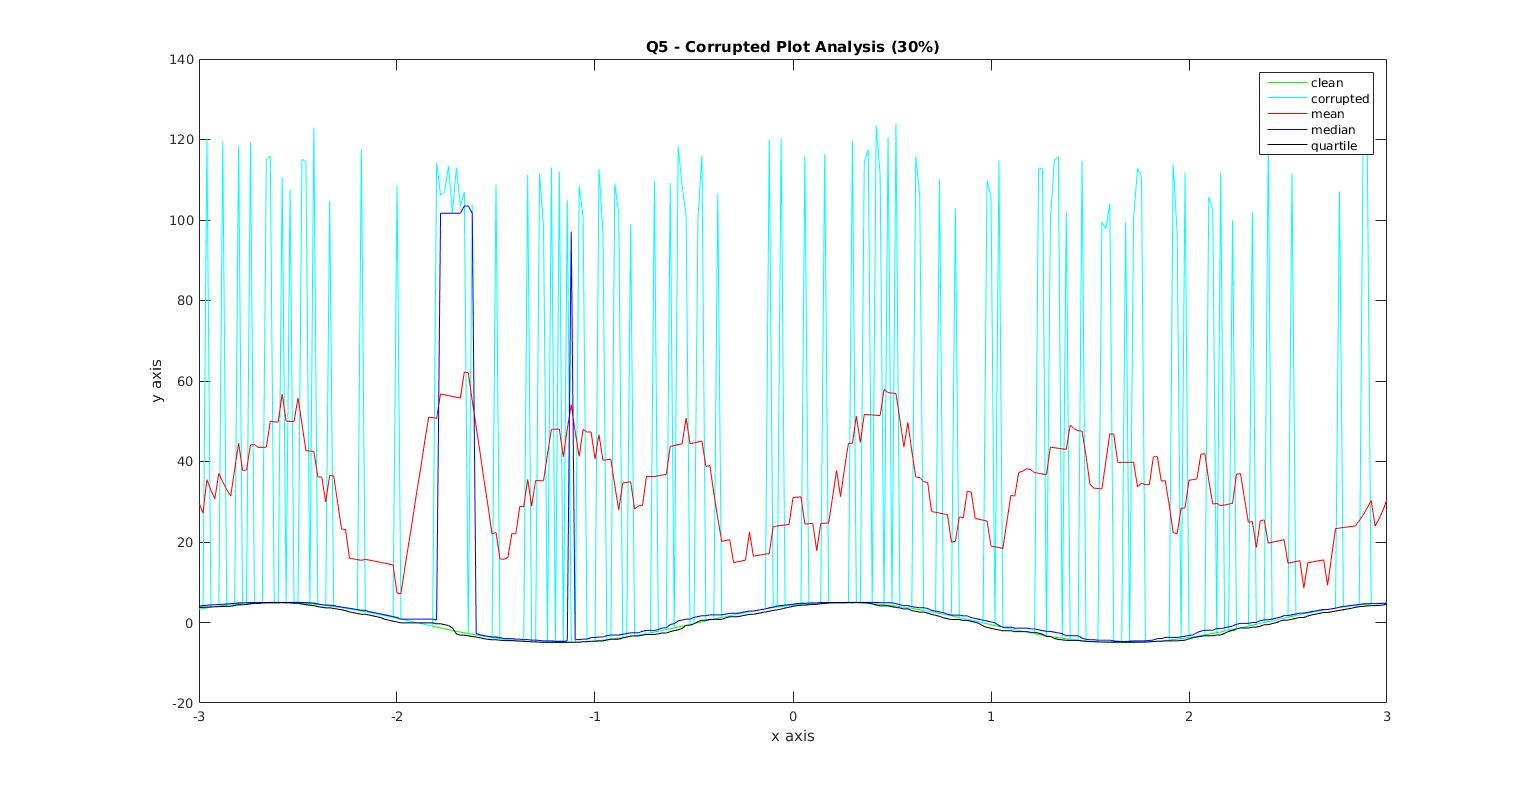
\includegraphics[width=\linewidth]{30.jpg}
	\caption{30\% data corrupted}
	\label{fig:5.1}
\end{figure}
\begin{figure}[h!]
	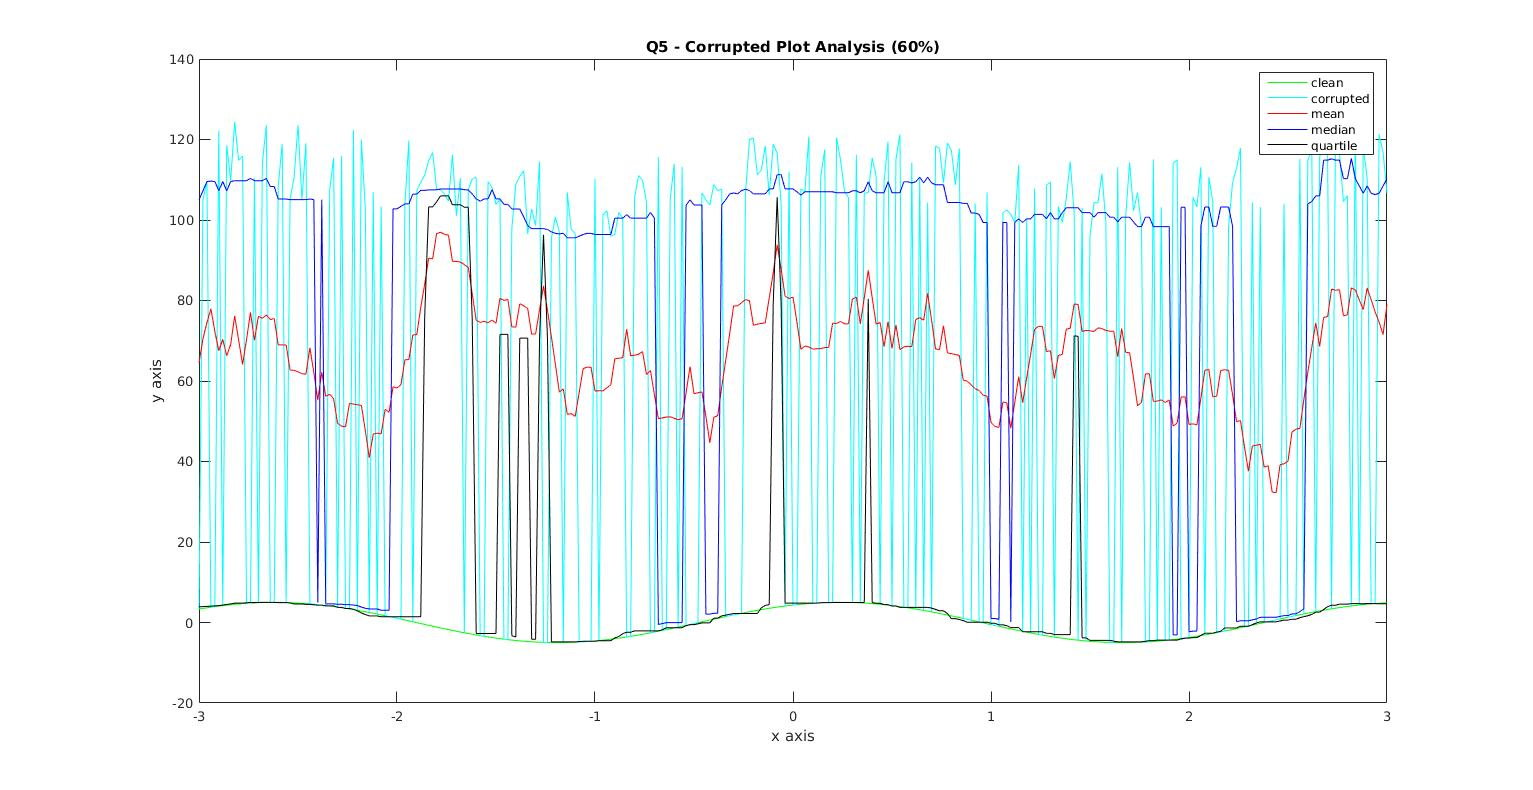
\includegraphics[width=\linewidth]{60.jpg}
	\caption{60\% data corrupted}
	\label{fig:5.2}
\end{figure}
\newpage
From the plots and the root mean square error data, it is clearly evident that the \textbf{moving quartile filtering} method has the \textbf{least root mean square error} and, hence, is the \textbf{best} method of filtering corrupted data.
\\ \\
This is because since the data is increased by around 100 when it is corrupted, we need to consider the smallest values in any interval while filtering. 


\textbf{Mean} of a data considers even the \textbf{corrupted values} and is heavily \textbf{influenced} by them. Hence we can safely rule out 'mean' as an optimum method for filtering.
 
 
\textbf{Median} of a data considers the middle term and is not influenced as heavily as mean by corruption but still, if \textbf{more than 50 \%} of the data is corrupted then the median will also be a \textbf{corrupted value}, and so we can rule out median as well.


\textbf{Quartile} of a dataset focusses on the lower 25\% data by value and we can say that it will \textbf{prioritize} \textbf{the clean (non corrupted) data} in any interval and hence will not get influenced by the corrupted data untill more than 75\% data in an interval has been corrupted.
\newline\newline
\textbf{Hence moving quartile filtering is the best way to filter our data.}

\newpage
\paragraph{Usage of MATLAB Code}
\begin{itemize}
\item Load code in the following path 'matlab\_code/q5/q5.m'
\item Run the code
\item This should output all values of root mean squared error for all three methods, both for 30\% corruption and 60\% corruption.
\item This should also generate two figures, one containing all the required plots for 30\%corruption and the other for 60\% corruption
\end{itemize}


\newpage
\section{Question 6}
Formulae for Updating the mean, median and standard deviation are :
\begin{enumerate}
\item The \textbf{updated} \textbf{Mean} is given by the following formula.
$$
Mean_{new} = \left(\frac{n.Mean_{old} + NewDataValue}{n+1}\right)
$$

\item For the \textbf{Updated Median}, given the variables $, Median_{old}$, number of Data \newline values(n), DataSet in increasing order, we consider the following cases.
\begin{alltt}
{\large\underline{Case I : n is even}}
      If NewDataValue \(\geq Median\sb{old}\)
            If NewDataValue \(\geq A\sb{\frac{n}{2}+1}\)
                  Median\(\sb{new} = A\sb{\frac{n}{2}+1}\)
            Else
                  Median\(\sb{new} = \)NewDataValue
      Else
            If NewDataValue \(\geq A\sb{\frac{n}{2}}\)
                  Median\(\sb{new} = \)NewDataValue
            Else
                  Median\(\sb{new} = A\sb{\frac{n}{2}}\)

{\large\underline{Case II : n is odd}}
      If NewDataValue \(\geq Median\sb{old}\)
            If NewDataValue \(\geq A\sb{\frac{n+1}{2}+1}\)
                  Median\(\sb{new} = \left(\frac{A\sb{\frac{n+1}{2}}+A\sb{\frac{n+1}{2}+1}}{2}\right)\)
            Else
                  Median\(\sb{new} = \left(\frac{A\sb{\frac{n+1}{2}}+NewDataValue}{2}\right)\)
      Else
            If NewDataValue \(\leq A\sb{\frac{n+1}{2}-1}\)
                  Median\(\sb{new} = \left(\frac{A\sb{\frac{n+1}{2}}+A\sb{\frac{n+1}{2}11}}{2}\right)\)
            Else
                  Median\(\sb{new} = \left(\frac{A\sb{\frac{n+1}{2}}+NewDataValue}{2}\right)\)

\end{alltt}

\item The updated \textbf{Standard Deviation }is given by the following formula.
$$
StD_{new} = \sqrt{\left(\frac{n(Mean_{old}-Mean_{new})^2 + (n-1)StD_{old}^2 + (NewDataValue - Mean_{old})^2}{n}\right)}
$$

\end{enumerate}
\newpage
\paragraph{Proofs}
\begin{enumerate}
\item {\Large\textbf {Mean}} \newline
\begin{equation} \label{eq:6.1}
Mean_{old} = \left(\frac{\sum_{i}a_i}{n}\right)
\end{equation}
$Similarly$
\begin{equation} \label{eq:6.2}
Mean_{new} = \left(\frac{\sum_{i}a_i + NewDataValue}{n+1}\right)
\end{equation}
Substituting value of $\sum_ia_i$ in eqn(~\ref{eq:6.2})
\begin{equation} \label{eq:6.3}
Mean_{new} = \left(\frac{n.Mean_{old} + NewDataValue}{n+1}\right)
\end{equation}

\item {\Large\textbf {Median}} \newline
\begin{equation*}
Median_{old} = \left\{
        \begin{array}{ll}
            \left(\frac{a_\frac{n}{2} + a_{\frac{n}{2}+1}}{2}\right) & \quad ; 2 | n \\
            a_\frac{n+1}{2} & \quad ;otherwise
        \end{array}
    \right\}
\end{equation*}
Now lets analyse all cases
\begin{itemize}
\item If the new value is equal to $Median_{old}$ then the new Median will be equal to $Median_{old}$ since Median is the 'Middle Element' and effectively, we are not adding any element greater or less than the median, so it will remain unchanged.
\item Lets now see for \textbf{even n}
	\begin{itemize}
	\item On adding an element, the number of elements will become odd, and hence the new median will be unique.
	\item The NewDataValue can either lie between the values of $a_\frac{n}{2}$ and $a_{\frac{n}{2}+1}$, or lie outside this range.
	\item If the NewDataValue lies between $a_\frac{n}{2}$ and $a_{\frac{n}{2}+1}$ then we can concur that in the new sequence (let it be b), the NewDataPoint will be $b_{\frac{n}{2} + 1}$ or $b_{\frac{n+1+1}{2}}$ which is the middle term, and hence the median.
	\item If the NewDataValue lies outside this range, then either of $a_\frac{n}{2}$ or $a_{\frac{n}{2}+1}$ will be the new median. Subsequently, if the new value is greater than the $Median_{old}$, then, $a_{\frac{n}{2}+1}$ will be the new Median, else, $a_{\frac{n}{2}}$ will be the new Median.
	\end{itemize}
	
\item Lets now see for \textbf{odd n}
	\begin{itemize}
	\item On adding an element, the number of elements will become even, and hence the new median will not be unique. (Lets say average of middle two terms)
	\item The NewDataValue can either lie between the values of $a_{\frac{n}{2}+1}$ and $a_{\frac{n}{2}-1}$, or lie outside this range.
	\item If the NewDataValue lies between $a_{\frac{n}{2}+1}$ and $a_{\frac{n}{2}-1}$, then the two middle values will comprise of the $Median_{old}$ and the NewDataValue itself, and hence the $Median_{new}$ will be an average of these two.
	\item If the NewDataValue lies outside this range, then the two middle values will comprise of the $Median_{old}$ and either of $a_{\frac{n}{2}+1}$ or $a_{\frac{n}{2}-1}$. Now if the NewDataValue is greater than $Median_{old}$ then the median will be the mean of $Median_{old}$ and $a_{\frac{n}{2}+1}$, else the $Median_{new}$ will be the mean of $a_{\frac{n}{2}-1}$ and $Median_{old}$.
	\end{itemize}
\end{itemize}

\item {\Large\textbf {Standard Deviation}} \newline
\begin{equation} \label{eq:6.4}
StD_{old} = \left(\sqrt{\frac{\sum_{i}(a_i-Mean_{old})^2}{n-1}}\right)
\end{equation}
$Similarly$
\begin{equation}\label{eq:6.5}
StD_{new} = \left(\sqrt{\frac{[\sum_{i}(a_i-Mean_{new})^2]+(NewDataValue-Mean_{new})^2}{n}}\right)
\end{equation}
Each term $(a_i - Mean_{new})$ can be written as $((a_i - Mean_{old}) + (Mean_{old} - Mean_{new}))$
\begin{equation}\label{eq:6.6}
StD_{new} = \left(\sqrt{\frac{[\sum_{i}((a_i - Mean_{old}) + (Mean_{old} - Mean_{new}))^2]+(NewDataValue-Mean_{new})^2}{n}}\right)
\end{equation}
We can simplify $\sum_i((a_i - Mean_{old}) + (Mean_{old} - Mean_{new}))^2$  as
\begin{equation*}
= \sum_i[(a_i - Mean_{old})^2 + (Mean_{old} - Mean_{new})^2 + 2(Mean_{old} - Mean_{new})(a_i - Mean_{old})]
\end{equation*}
\begin{equation*}
= \sum_i[(a_i - Mean_{old})^2] + \sum_i[(Mean_{old} - Mean_{new})^2] + \sum_i[2(Mean_{old} - Mean_{new})(a_i - Mean_{old})]
\end{equation*}
\begin{equation*}
= \sum_i[(a_i - Mean_{old})^2] + n.(Mean_{old} - Mean_{new})^2 + \left\{2(Mean_{old} - Mean_{new})\sum[(a_i - Mean_{old})]\right\}
\end{equation*}
Now since $\sum[(a_i - Mean_{old})] = 0$, we get
\begin{equation*}
= \sum_i[(a_i - Mean_{old})^2] + n.(Mean_{old} - Mean_{new})^2
\end{equation*}
Substituting eqn(~\ref{eq:6.4}), we get
\begin{equation}\label{eq:6.7}
= (n-1)StD_{old}^2 + n.(Mean_{old} - Mean_{new})^2
\end{equation}
Substituting eqn(~\ref{eq:6.7}) in eqn(~\ref{eq:6.6}), we get,
\begin{equation}\label{eq:6.8}
StD_{new} = \left(\sqrt{\frac{(n-1)StD_{old}^2+n(Mean_{old}-Mean_{new})^2+(NewDataValue-Mean_{new})^2}{n}}\right)
\end{equation}
Hence Proved!
\end{enumerate}

\paragraph{Usage of MATLAB Code}
\begin{itemize}
\item Load code in the following path 'matlab\_code/q6/'
\item There should be three different matlab files corresponding to the required three fucntions
\item This is done since MATLAB versions <2016 do not support function declarations in a single script file
\item Load and run every function in the command line window for testing
\end{itemize}
\paragraph{Updating the Histogram\newline}
Let the frequency be plotted on the y axis.\newline
Then increase the value of frequency corresponding to the new data value by 1.\newline


\newpage
\section{Question 7}
\textbf{Formula}
\newline
The number of people 'n' such that any two of them have the same birthday with atleast 'p' probability is given by the inequality
$$\left(1-\frac{^{365}C_n}{365^n}\right) \leq p$$
The situation can be visualized as the negation of the event where all n people have unique birthdays.
\newline
The plot of values of n vs p is given in Figure~\ref{fig:7.1}
\begin{flushright}
$\forall$ p $\in \{5, 10, 15, 20, 30, 40, 50, 60, 70, 80, 90, 95, 99, 99.99, 99.9999, 100\}$
\end{flushright}
\begin{figure} [h!]
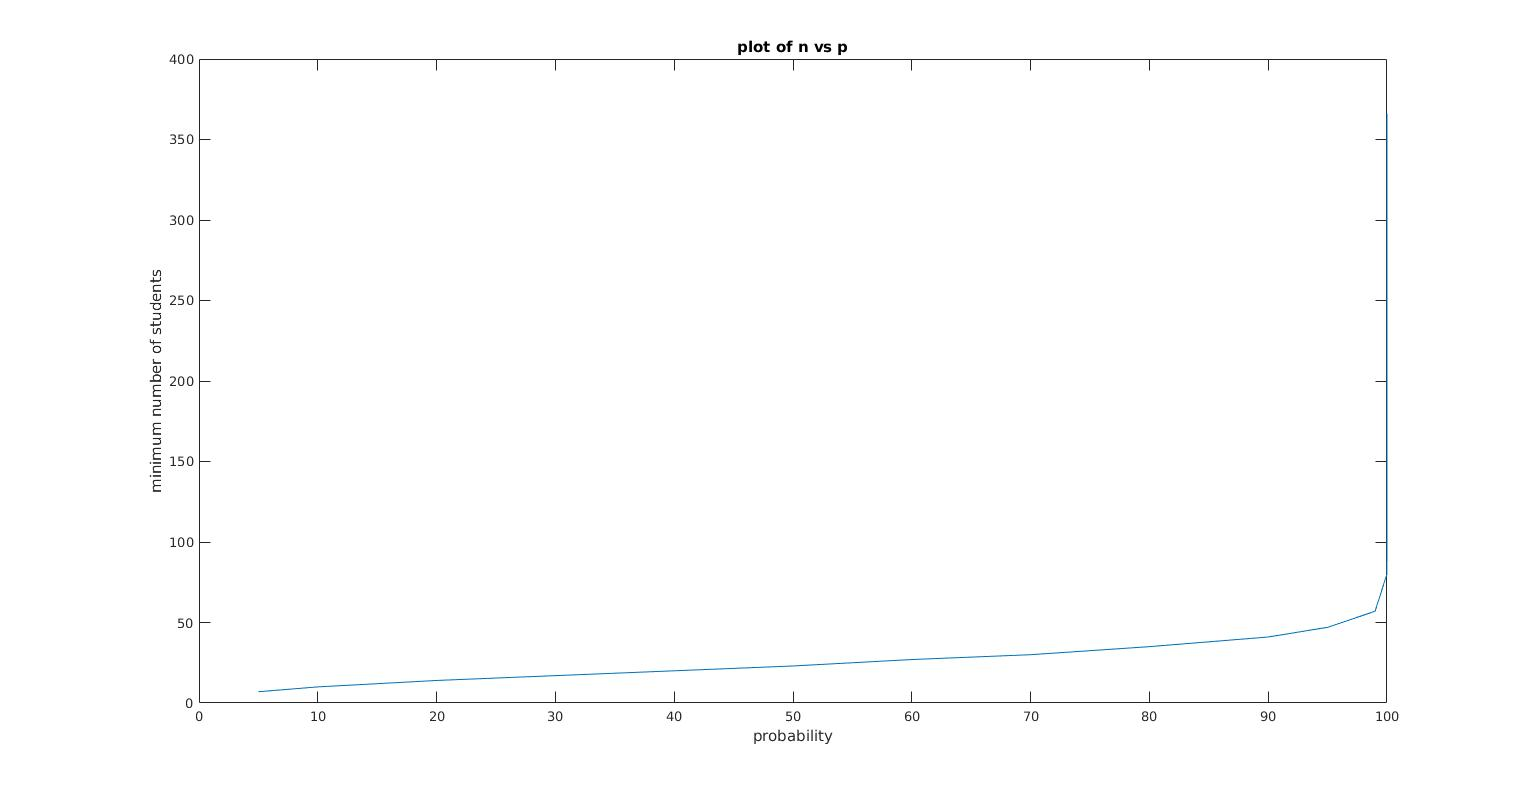
\includegraphics[width=\linewidth]{plot.jpg}
\caption{plot of n vs p}
\label{fig:7.1}
\end{figure}
\textbf{Usage of the MATLAB Code}
\begin{itemize}
\item Load code in the following path 'matlab\_code/q5/q5.m'
\item Run the code
\item This should output all values of n for corresponding values of p
\item This should also plot the required plot of n vs p
\end{itemize}

\end{document}